\def\currentRootFolder{chapter/energyDependentCrossSec}
\def\currentFigureFolder{\currentRootFolder/fig}
\newcommand{\sigmaInel}{\sigma_\mathrm{inel}}
\newcommand{\sigmaAvg}{\sigma_\mathrm{avg}}

\newcommand{\qUmin}{qU_\mathrm{min}}

\newcommand{\Ekin}{E_\mathrm{kin}}
\newcommand{\nSource}{n_\mathrm{S}}
\newacronym{standardmodel}{SM}{Standard Model of Particle Physics}
\newacronym{lep}{LEP}{Large Electron Positron Collider}
\newacronym{ssm}{SSM}{standard solar model}
\chapter{Energy-Dependence of the Cross Section for Inelastic Electron-Scattering within the \glsentryshort{wgts}}
\label{sec:eDepScatCrossSec}
The probability for an electron to scatter when traveling through the \gls{wgts} can be characterized by the total scattering cross section $\sigma_\mathrm{tot}$. Two types of scatterings can be distinguished: elastic and inelastic scattering. The cross section for elastic scattering is smaller than the one for inelastic scattering by one order of magnitude~\cite{Kleesiek2019} (also see~\ref{sec:intSpecModelResponseEloss} for a comparison of th cross section values). This chapter focuses on inelastic scattering and neglects elastic scattering. Within this chapter, the cross section for electrons scattering inelastically off gas molecules is just denoted as ``cross section'' and with the symbol $\sigma$. For ease of notation and reading, the adjective ``inelastic'' and an index such as ``inel'' is omitted where the context allows it unambiguously.

The cross section depends on the energy of the incident electrons: $\sigma \equiv \sigma(E)$. This dependence has been neglected in the formal modeling of a KATRIN measurement described in chapter~\ref{sec:intSpecModel}. This chapter investigates effects related to the incorporation of the energy-dependence. Section~\ref{sec:eDepScatCrossSecSources} lists cross section values and formulae from different sources and relates them to each other. Section~\ref{sec:eDepScatCrossSecModelPoisson} extends the mathematical formalism for a KATRIN measurement in order to incorporate the energy-dependence of the scattering cross section. However, an approximation is made. It is neglected, that an electron that scatters loses energy and becomes more likely to scatter again. This issue is addressed in section~\ref{sec:eDepScatCrossSecModelExtended}. Section~\ref{sec:eDepScatCrossSecNuMassInf} discusses the energy-dependence of the scattering cross section within the context of neutrino mass inference using the approximated model. And section~\ref{sec:eDepScatCrossSecConclusion} concludes and offers an outlook.


\section{Cross Section Values for Inelastic Electron-Scattering off Molecular Hydrogen Isotopologues}
\label{sec:eDepScatCrossSecSources}
The goal of this thesis is to investigate to what extend it is important, that the cross section value is not constant but varies with the energy of the incident electrons. In that regard, a formula by~\cite{Liu1987} is used, that is derived from first principles and denotes the energy-dependent cross section for electrons scattering off hydrogen molecules. This was found to be a feasible approach for the stated goal - at least for first investigations. In section~\ref{sec:eDepScatCrossSecSourcesTheory}, this formula by~\cite{Liu1987} is reviewed. For electrons with an energy of $\Esource=\SI{18.6}{keV}$, its application yields 
\begin{equation}
	\label{eq:eDepScatCrossSecSourcesCrossSecLiuAtEndpoint}
	\sigma(\SI{18.6}{keV}) = \SI{3.667e-22}{m^2}
	\fullstop
\end{equation}
The formula is in agreement on at least the $10^{-1}$ level with recent, preliminary estimations obtained through data taken at the KATRIN experiment for electrons scattering off tritium molecules. This hints at its applicability, which is of importance in the light of the following paragraph.

The situation regarding cross section values is not without a certain intricacy. The following list gives an introduction to the matter that shall serve as guidance for the reader:\mynobreakpar
\begin{enumerate}
	\item In this work, a theoretical cross section for electrons scattering off hydrogen molecules is used. During a KATRIN neutrino mass measurement, the \gls{wgts} is envisaged to be filled with gas of \SI{95}{\percent} tritium purity~\cite{Angrik:2005ep}. In that regard, the scattering off tritium molecules is of importance with respect to the KATRIN experiment. How the formulas for scattering off hydrogen molecules can be transformed to tritium molecules is under investigation at the time of writing this thesis. Once, this process is completed, the study presented in this thesis might have to be repeated.
	\item The cross section for electrons with an energy of \SI{18.6}{keV} scattering off tritium molecules was measured at the neutrino mass experiment in Troitsk to be~\cite{Aseev2000}
	\begin{equation}
		\sigma(\SI{18.6}{eV}) = \SI{3.40\pm0.07e-22}{m^2}
		\fullstop
	\end{equation}
	This value differs by approximately \SI{8}{\percent} and 4 standard deviations from the theoretical value given above in equation~\eqref{eq:eDepScatCrossSecSourcesCrossSecLiuAtEndpoint}.
	\item The KATRIN Design Report lists a reference value~\cite{Angrik:2005ep}
	\begin{equation}
	\label{eq:eDepScatCrossSecSourcesCrossSecTDR}
	\sigma_\mathrm{TDR} = \SI{3.456e-22}{m^2}
	\fullstop
	\end{equation}
	This value also differs significantly from the theoretical value given above in equation~\eqref{eq:eDepScatCrossSecSourcesCrossSecLiuAtEndpoint}. To further complicate the matter, comparability with former results is of importance in the scope of this thesis and several former works are based on $\sigma_\mathrm{TDR}$. Section~\ref{sec:eDepScatCrossSecSourcesChoice} explains why the value of $\sigma_\mathrm{TDR}$ might be erroneous and how this issue is addressed in this work.
\end{enumerate}

\subsection{Theoretical Cross Section Formulae}
\label{sec:eDepScatCrossSecSourcesTheory}
An expression for the inelastic cross section for electrons scattering off hydrogen molecules can be found in~\cite{Liu1973}. Two expressions are given: one for relativistic incident electrons and one for non-relativistic incident electrons. In regard to KATRIN, the energies of $\upbeta$~electrons from tritium $\upbeta$~decay are relevant. The maximum relativistic $\beta$~factor of electrons from tritium $\upbeta$~decay is
\begin{align}
\beta(E, m) &= 
\sqrt{
	1-\frac{1}{
		(\frac{E}{m}+1)^2
	}
} \label{eq:eDepScatCrossSecSourcesCrossSecBetaFactor} \\
\Rightarrow\beta_\mathrm{max, T} &= 
\beta(E\approx\SI{18.6}{keV}, m_\elecIndex\approx\SI{511}{keV})\approx0.26 
\fullstop
\end{align}
Traveling at approximately a forth of the speed of light, the $\upbeta$~electrons are assumed to behave non-relativisticly. Then, the given expression for the energy-dependent cross section is~\cite{Liu1973}
\begin{equation}
\label{eq:eDepScatCrossSecSourcesCrossSecLiu}
\sigma(E) =  
(4 \pi a_0^2) \cdot
\left(\frac{T(E)}{R}\right)^{-1} \cdot
\left[
C_1 \cdot \ln{\left(\frac{T(E)}{R}\right)} + C_2
\right]
\end{equation}
with the Bohr radius\footnote{Bohr radius $a_0=\SI[separate-uncertainty=false]{0.529 177 210 67(12)e-10}{m}$~\cite{ReviewOfParticlePhysics}} $a_0$, 
the Rydberg energy\footnote{Rydberg energy $R=\SI[separate-uncertainty=false]{13.605 693 009(84)}{eV}$~\cite{ReviewOfParticlePhysics}} $R$ and two constants $C_1$ and $C_2$. The later two depend on the hydrogen isotopologue. Different values are stated in different works for scattering off hydrogen molecules
\begin{subequations}
\label{eq:eDepScatCrossSecSourcesCrossSecLiuConstants}
\begin{align}
C_1 &= 1.5487 &&\text{\cite{Liu1973}}
\label{eq:eDepScatCrossSecSourcesCrossSecLiuConstantsC1}
\comma\\[10pt]
C_2 &= 2.2212\pm0.0434 &&\text{\cite{Liu1973}}
\label{eq:eDepScatCrossSecSourcesCrossSecLiuConstantsC2Uncert}
\comma\\
C_2 &= 1.53 &&\text{\cite{Gerhart1975}}
\comma\\
C_2 &= 2.4036 &&\text{\cite{Liu1987}}
\label{eq:eDepScatCrossSecSourcesCrossSecLiuConstantsC2}
\fullstop
\end{align}
\end{subequations}
The latest of these references,~\cite{Liu1987}, acknowledges that the listed values for $C_2$ are not compatible.

Furthermore, in equation~\eqref{eq:eDepScatCrossSecSourcesCrossSecLiu}, $T$ denotes the classical kinetic energy\footnote{I would like to thank Dr.~F. Glück for pointing this out. Also see~\cite{INOKUTI1971} for notations with regard to Bethe theory in scattering processes.} using the velocity $v$ and the electron rest mass $m_\elecIndex$
\begin{align}
	\label{eq:eDepScatCrossSecSourcesCrossSecNonRelEnergy}
	T  &= \frac{1}{2} m_\elecIndex v^2 = 
	\frac{1}{2} m_\elecIndex  c^2  \frac{v^2}{c^2} \nonumber \\
	&\equiv T(E) = \frac{1}{2} m_\elecIndex  c^2  \beta(E, m_\elecIndex)^2
\end{align}
with $\beta(E, m_\elecIndex)$ as in equation~\eqref{eq:eDepScatCrossSecSourcesCrossSecBetaFactor}\footnote{This thesis uses natural units. However, for clarity, it makes sense to explicitly state the speed of light $c$ in this particular case.}. This formula is valid in the center-of-mass frame of the colliding system of the electron and the hydrogen molecule. As the molecule is significantly heavier than an electron, the center of mass-frame-was assumed to be the rest frame of the molecule. Also, relative movements due to the gas flow and thermal motion in the \gls{wgts} were neglected.

In the scope of this thesis, equation~\eqref{eq:eDepScatCrossSecSourcesCrossSecLiu} with $C_2$ from~\cite{Liu1987} (as it is the most up-to-date of the listed ones) is used to include the energy-dependence of the cross section into the mathematical formalism of a KATRIN neutrino mass measurement.

In \cite{Liu1973}, also a formula for incident electrons with relativistic energies is given. As already mentioned, in this thesis, the $\upbeta$ electrons from tritium decay are assumed to behave non-relativisticly and the formula is only reprinted here for completeness
\begin{equation}
	\label{eq:eDepScatCrossSecSourcesCrossSecLiuRelativistic}
	\sigma(E) =  
	(4 \pi a_0^2) \cdot
	\left(\frac{T(E)}{R}\right)^{-1} \cdot
	\left[
	1.5487 \cdot \ln{\left(\frac{\beta(E,m_\elecIndex)}{1-\beta(E,m_\elecIndex)^2}\right)} + 17.4615
	\right]
	\fullstop
\end{equation}
The quantities $T(E)$, $R$ and $a_0$ match the once in equation~\eqref{eq:eDepScatCrossSecSourcesCrossSecLiu} and $\beta(E, m_\elecIndex)$ follows equation~\eqref{eq:eDepScatCrossSecSourcesCrossSecBetaFactor}. For energies below $\SI{18.6}{keV}$ the difference of the formula for relativistic (eq.~\ref{eq:eDepScatCrossSecSourcesCrossSecLiu}) and non-relativistic (eq.~\ref{eq:eDepScatCrossSecSourcesCrossSecLiuRelativistic}) incident electrons is less than \SI{1}{\percent}. To what extend relativistic effects in the inelastic scattering process could be of relevance for the KATRIN experiment is not covered in this thesis.

Figure~\ref{fig:eDepScatCrossSecSourcesValues} shows the theoretical cross-section formulae~\eqref{eq:eDepScatCrossSecSourcesCrossSecLiu} and~\eqref{eq:eDepScatCrossSecSourcesCrossSecLiuRelativistic} along with the measured value by the Troitsk experiment and the reference value from the KATRIN Design Report.

\begin{figure}[t]
	\centering
	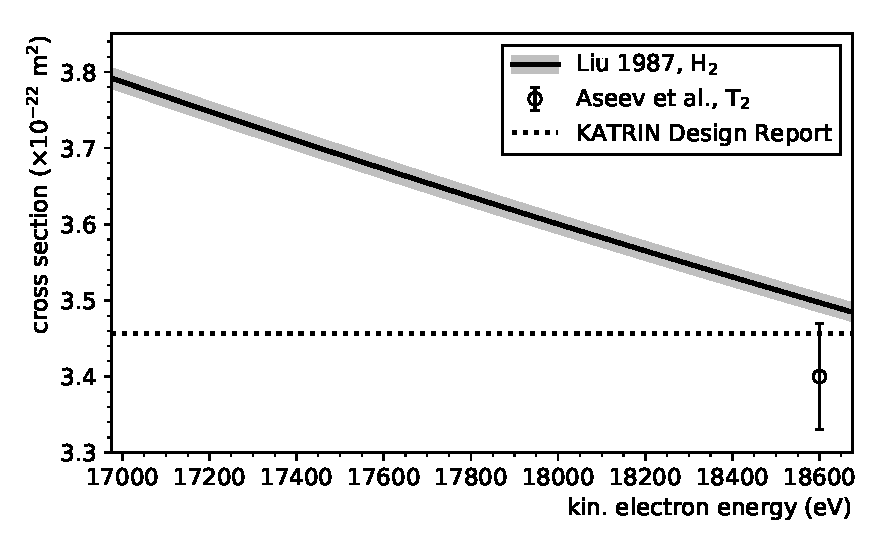
\includegraphics[width=\textwidth]{\currentFigureFolder/crossSecNoZoom.pdf}
	\xcaption{Inelastic cross section for electrons scattering off molecular hydrogen isotopologues}{Inelastic cross section for electrons scattering off molecular hydrogen isotopologues.}{The continuous line shows equation~\eqref{eq:eDepScatCrossSecSourcesCrossSecLiu} for incident electrons with non-relativistic energies with constants from equation~\eqref{eq:eDepScatCrossSecSourcesCrossSecLiuConstantsC1} and~\eqref{eq:eDepScatCrossSecSourcesCrossSecLiuConstantsC2} where the later is assumed to have an uncertainty according to equation~\eqref{eq:eDepScatCrossSecSourcesCrossSecLiuConstantsC2Uncert}. The dashed line shows equation~\eqref{eq:eDepScatCrossSecSourcesCrossSecLiuRelativistic} for incident electrons with relativistic energies. Also, the measurement by~\cite{Aseev2000} at the Troitsk neutrino mass experiment and the value stated in the KATRIN Design Report~\cite{Angrik:2005ep} are depicted. The shown energy interval is chosen according to the \gls{mtd} of the \gls{ft} measurement campaign.}
	\label{fig:eDepScatCrossSecSourcesValues}
\end{figure}

\subsection{Relation to Cross Section Values Used in Former Works}
\label{sec:eDepScatCrossSecSourcesChoice}
As already stated and depicted in figure~\ref{fig:eDepScatCrossSecSourcesValues}, the reference cross section from the KATRIN Design Report does not match the theoretical calculations used in this thesis. Nonetheless, several former works (see subsequent section~\ref{sec:eDepScatCrossSecNuMassInf}) are based on the reference value. Comparability is of importance in the scope of this thesis (as will become apparent in section~\ref{sec:eDepScatCrossSecNuMassInf}). How this issue is addressed is explained in the following.

The cross section value stated in the KATRIN Design Report can be recovered from equation~\eqref{eq:eDepScatCrossSecSourcesCrossSecLiu} if an erroneous energy interpretation is applied. If, instead of equation~\eqref{eq:eDepScatCrossSecSourcesCrossSecNonRelEnergy}, one applies the energy interpretation
\begin{equation}
	\label{eq:eDepScatCrossSecSourcesCrossSecTDREngeryInterpretation}
	T(E) = E
	\comma
\end{equation}
the obtained cross section via equation~\eqref{eq:eDepScatCrossSecSourcesCrossSecLiu} is
\begin{equation}
\label{eq:eDepScatCrossSecSourcesTRDCrossSec}
	\sigma_\mathrm{TDR} 
	\equiv\sigma(E_\mathrm{TDR}=\SI{18565}{eV})
	=\SI{3.4559e-22}{m^2} 
	\approx\SI{3.456e-22}{m^2}
\end{equation}
as stated in the KATRIN Design Report, where the energy $E_\mathrm{TDR}$ is approximately central in the KATRIN design analysis interval (see section~\ref{sec:intSpecModelMTD}). Whether this had been the approach, that had led to the reference cross section in the KATRIN Design Report is not known. 

This work applies the energy interpretation~\eqref{eq:eDepScatCrossSecSourcesCrossSecTDREngeryInterpretation} when comparability to former works, that used the reference cross section from the KATRIN Design Report, is of importance. Otherwise, equation~\eqref{eq:eDepScatCrossSecSourcesCrossSecNonRelEnergy} is used. Corresponding indications are given on a case to case basis. The quantitative difference of these two approaches can be assessed by expanding the $\beta$-factor~\eqref{eq:eDepScatCrossSecSourcesCrossSecBetaFactor} in the ratio $E/m_\elecIndex \approx 18.575/511 \approx 0.036 \ll 1$
\begin{equation}
	\beta^2 \approx 
	2 \frac{E}{m_\elecIndex} - 
	3 \left(\frac{E}{m_\elecIndex}\right)^2
	\fullstop
\end{equation}
The energy interpretation of equation~\eqref{eq:eDepScatCrossSecSourcesCrossSecNonRelEnergy} then becomes
\begin{equation}
	T(E) \approx 0.95 \cdot E
	\comma
\end{equation}
which is a shift in energy and hence, in first order, also in the cross section of about \SI{5}{\percent} compared to the interpretation in equation~\eqref{eq:eDepScatCrossSecSourcesCrossSecTDREngeryInterpretation}. Exact calculations are given in table~\ref{tab:eDepScatCrossSecModelScatProbs}.

\section{An Energy-Dependent Scattering Model using the Poisson Distribution}
\label{sec:eDepScatCrossSecModelPoisson}
The energy-dependence of the cross section enters into the calculation of the scattering probabilities~\eqref{eq:intSpecModelNonAveragedScatProbs}. In the derivation that is given in the previous section~\ref{sec:intSpecModelResponseScattering} the dependence on the starting energy $\Esource$ of electrons is neglected. Instead, an average starting energy and hence an average scattering cross section
\begin{equation}
	\sigma_\mathrm{TDR}(E_\mathrm{TDR})=\SI{3.456e-22}{m^2}
\end{equation}  (energy interpretation as per equation~\ref{eq:eDepScatCrossSecSourcesCrossSecTDREngeryInterpretation}) is assumed. Table~\ref{tab:eDepScatCrossSecModelScatProbs} lists the corresponding scattering probabilities averaged over all starting positions and pitch angles of electrons. Additionally, the results of a Monte Carlo particle tracking simulation by~\cite{Groh2015} and the values using the energy interpretation of equation~\eqref{eq:eDepScatCrossSecSourcesCrossSecNonRelEnergy} are given. How, instead of assuming energy-independent scattering probabilities, the energy-dependence can be modeled is shown in the following.
\begin{table}[t]
	\centering
	\xcaption{Probability for severalfold electron-scattering in the \glsentryshort{wgts} - reviewed}{Probability for severalfold electron-scattering in the \glsentryshort{wgts}.}{The probabilities are averaged over all starting positions and starting pitch angles. Both, the values from a Monte Carlo (MC) particle tracking simulation and the values according to equation~\eqref{eq:intSpecModelAveragedScatProbs} are given. The  cross section was evaluated at an energy of $E_\mathrm{TDR}=\SI{18564.37463}{eV}$ for the two energy interpretations described by equation~\eqref{eq:eDepScatCrossSecSourcesCrossSecTDREngeryInterpretation} and~\eqref{eq:eDepScatCrossSecSourcesCrossSecNonRelEnergy}. Further input parameters to the calculations are a constant gas column density $\rho d = \SI{5e17}{cm^{-2}}$, 
	a \gls{wgts} length of $d=\SI{10.0820}{m}$
	and a maximum acceptance angle of $\thetaMax=\SI{50.7685}{\degree}$. The values are given with the precision needed to reproduce the results in the table below in all digits, which is the precision used in \glsentryshort{ssc}. The energy is chosen such, that $\sigma_\mathrm{TDR}=\SI{3.456000e-22}{m^2}$ is recovered in more than 3 digits as per equation~\eqref{eq:eDepScatCrossSecSourcesTRDCrossSec}.}
	\begin{tabular}{lllr}
		\toprule
		\makecell[tl]{cross section (\SI{e-22}{m^2}) $\rightarrow$} &
		3.456 &
		3.456 &
		3.673 \\
		\hline
		\makecell[tl]{source $\rightarrow$} & 
		\makecell[tl]{MC particle tracking\\ \cite{Groh2015}} & 
		\makecell[tl]{eq.~\eqref{eq:intSpecModelAveragedScatProbs} \\ \cite{Groh2015, Kleesiek2014}} &
		\makecell[tr]{eq.~\eqref{eq:intSpecModelAveragedScatProbs}}
		\\
		\hline
		\makecell[cl]{scattering count $\downarrow$} & 
		& 
	    & \\
		\hline
		\makecell{0} & $0.415 \pm 0.002$ & 0.41334 & 0.39564 \\
		\makecell{1} & $0.292 \pm 0.002$ & 0.29266 & 0.28967 \\
		\makecell{2} & $0.166 \pm 0.001$ & 0.16733 & 0.17298 \\
		\makecell{3} & $0.079 \pm 0.001$ & 0.07913 & 0.08590 \\
		\makecell{4} & $0.031 \pm 0.001$ & 0.03178 & 0.03634 \\
		\bottomrule
	\end{tabular}
	\label{tab:eDepScatCrossSecModelScatProbs}
\end{table}

\begin{figure}[th]
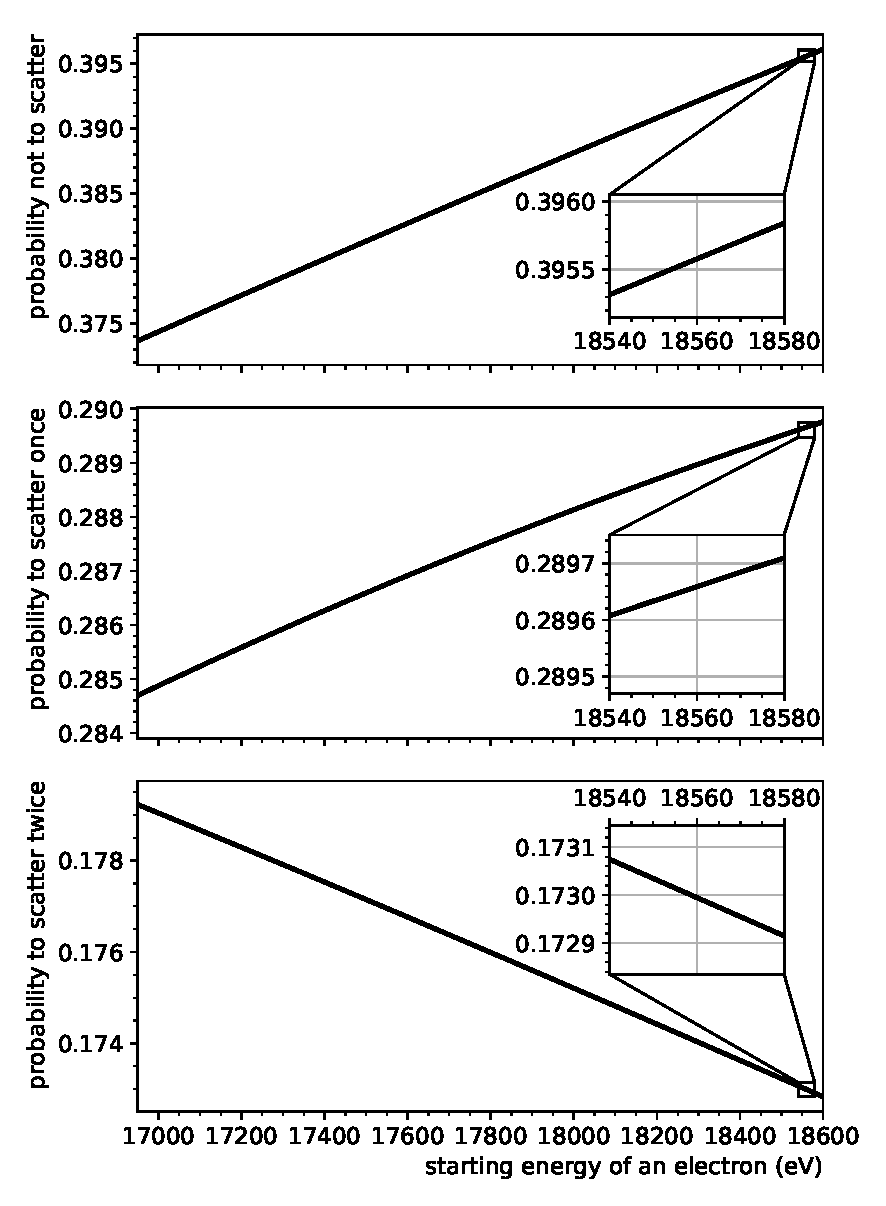
\includegraphics[width=\textwidth]{\currentFigureFolder/scatProbs012Poisson.pdf}
        \xcaption{Probability for severalfold electron-scattering in the \glsentryshort{wgts}}{Probability for severalfold electron-scattering in the \glsentryshort{wgts}.}{From top to bottom, the probability for no, one-fold and two-fold scattering are shown averaged over all starting positions and starting pitch angles of electrons in the \gls{wgts} according to the Poisson Model in equation~\eqref{eq:eDepScatCrossSecModelPoisson}. The shown energy range matches the measurement range of the \gls{ft} measurement campaign and the inset shows an energy span around the endpoint of the tritium $\upbeta$~spectrum.}
        \label{fig:eDepScatCrossSecModel}
\end{figure}

\subsection{Formalism of the Poisson Model for Electron-Scattering}
An expression for the probability of $l$-fold scattering of electrons within the \gls{wgts} is derived in the previous section~\ref{sec:intSpecModelResponseScattering}. The given model is independent of the energy of the electrons. Instead of using a constant cross section, the energy-dependence can be respected. The corresponding formulae from section~\ref{sec:intSpecModelResponseScattering} are repeated below with the energy-dependence made explicit and by using an energy-dependent cross section as per equation~\eqref{eq:eDepScatCrossSecSourcesCrossSecLiu}
\begin{subequations}
\label{eq:eDepScatCrossSecModelPoisson}
\begin{align}
    \mu(\Esource,\zSource,\thetaSource) =&
    \frac{\sigma(\Esource)}{\cos\thetaSource}
    \int_{\zSource}^{d/2} \rho(z)\d z \label{eq:energydepScatProbsPoissonExpectedScatCount} 
    \comma\\
    P_l(\Esource,\zSource,\thetaSource) =&
    \mathrm{Poisson}(\mu(\Esource,\zSource,\thetaSource),l) \label{eq:eDepScatCrossSecModelPoissonNonAveragedScatProbs} 
    \comma \\
    \bar{P}_l(\Esource) =&
    \frac{1}{d \cdot (1-\cos(\thetaMax))} 
      \int_{-d/2}^{d/2}  
          \int_{0}^{\theta_{max}} 
            \sin(\thetaSource)
            \mathrm{Poisson}(\mu(\Esource,\zSource,\thetaSource),l)
          \d\thetaSource
      \d\zSource
      \label{eq:eDepScatCrossSecModelPoissonAveragedScatProbs}
    \fullstop
\end{align}
\end{subequations}
As a reminder, $\bar{P}_l(\Esource)$ in equation~\eqref{eq:eDepScatCrossSecModelPoissonAveragedScatProbs} denotes the probability for $l$-fold scattering of an electron with a starting kinetic energy $\Esource$ averaged over all starting positions and pitch angles in the \gls{wgts}. In the following, this model is denoted ``Poisson model''. 

\subsection{Properties of the Poisson Model for Electron-Scattering}
\label{sec:eDepScatCrossSecModelPoissonProperties}
Figure~\ref{fig:eDepScatCrossSecModel} shows the Poisson model as per equation~\eqref{eq:eDepScatCrossSecModelPoisson}. Table \ref{tab:eDepScatCrossSecModelScatProbs} lists the scattering probabilities for an energy-independent Poisson model (see section~\ref{sec:intSpecModelResponseScattering}) and a reference cross section $\sigma(E\approx\SI{18564}{eV})=\SI{3.673e-22}{m}$. The energy-dependent Poisson model recovers the energy-independent model exactly at the corresponding energy as expected.

\paragraph{Trend of the Energy-Dependence}
\begin{figure}[th]
	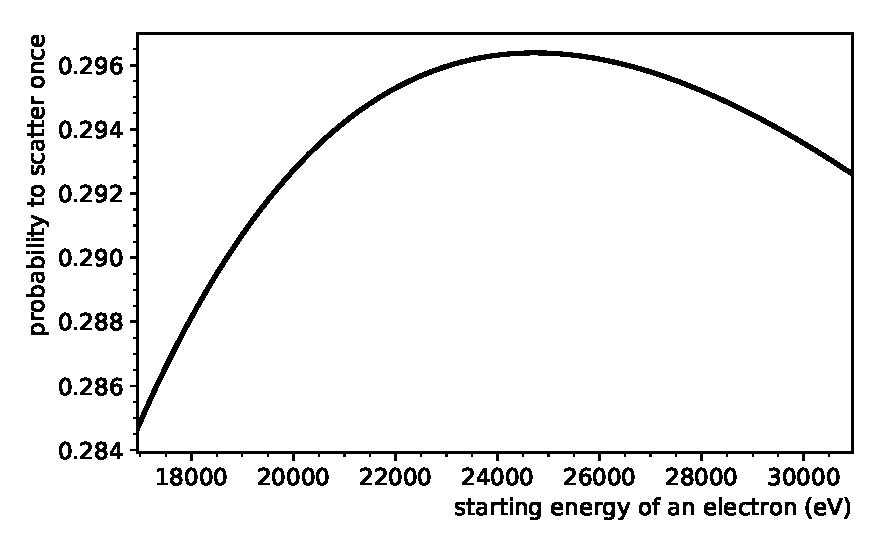
\includegraphics[width=\textwidth]{\currentFigureFolder/scatProbs1Poisson_extendedEnergyRange.pdf}
	\xcaption{Probability for one-fold electron-scattering in the \glsentryshort{wgts} in an extended energy range}{Probability for one-fold electron-scattering in the \glsentryshort{wgts} in an extended energy range.}{The graph shows the probability of one-fold scattering according to equation~\eqref{eq:eDepScatCrossSecModelPoissonAveragedScatProbs}. It emphasizes the change of sign in the derivative at approximately \SI{24.7}{keV}.}
	\label{fig:eDepScatCrossSecModelPoissonP1ExtendedEnergyRange}
\end{figure}
As depicted in figure~\ref{fig:eDepScatCrossSecModel}, for an increasing starting energy of electrons within the \gls{wgts}, the probability for no and one-fold scattering also increases, while the probability for two-fold scattering decreases. This paragraph aims to give an intuitive argument for this change of sign in the derivative $\d \bar{P}_l(\Esource) / \d \Esource$ in the transition from $l=1$ to $l=2$. The Poisson model $\bar{P}_l(\Esource)$ is a probability density in $l$ for a fixed $\Esource$ (see appendix~\ref{sec:appendixEDepScatCrossSecPoissonModelProbDensityProof} for a proof). Hence, the expected scattering count for an energy within the range of starting energies $\Esource \in [\SI{17}{keV}, \SI{18.6}{keV}]$, that is depicted in figure~\ref{fig:eDepScatCrossSecModel}, can be calculated (numerically)
\begin{equation}
\label{eq:eDepScatCrossSecModelPoissonExpectedScatCount}
\begin{split}	
	\bar{l}(\SI{17.0}{keV}) &= 
	\sum_{l}^{\infty} \bar{P}_l(\SI{17.0}{keV}) \cdot l \approx 1.23 \\	
	\bar{l}(\SI{18.6}{keV}) &= 
	\sum_{l}^{\infty} \bar{P}_l(\SI{18.6}{keV}) \cdot l \approx 1.14
	\fullstop
\end{split}
\end{equation} 
In other words, electrons with a starting energy between \SI{17}{keV} and \SI{18.6}{keV} are expected to scatter between 1 and 2 times on their way through the \gls{wgts} (averaged over all starting positions and pitch angles). Then, the illustrative line of argument is the following: 
\begin{align*}
	&\text{ the starting energy $\Esource$ increases} \\ \Rightarrow
	&\text{ the scattering cross section decreases (see figure~\ref{fig:eDepScatCrossSecSourcesValues})} \\ \Rightarrow
	&\text{ scattering becomes less likely} \\ \Rightarrow
	&\text{ $\bar{l}$ decreases and moves closer to 1 and away from 2} \\ \Rightarrow
	&\text{ the probability for no and one-fold scattering increases,} \\
	&\text{ while the probability for more than one scattering decreases}
	\fullstop
\end{align*} 
This is in accordance with the trend of the energy-dependence depicted in figure~\ref{fig:eDepScatCrossSecModel}. Also, if this reasoning is correct, the sign of $\d \bar{P}_1(\Esource) / \d \Esource$ for one-fold scattering should change for sufficiently high energies and the probability to scatter once should decrease. This is indeed the case as depicted in figure~\ref{fig:eDepScatCrossSecModelPoissonP1ExtendedEnergyRange}. The decrease starts at an energy of roughly \SI{24.7}{keV}. This might for example be of relevance for the measurement of Krypton conversion lines in calibration measurements because the corresponding electron energies are above \SI{30}{keV}~\cite{venos2018}.


\paragraph{Limit of the Poisson Model for Electron-Scattering}
The Poisson model is exact for the probability of no scattering $\bar{P}_0(\Esource)$, but it does not hold for one or more scatterings because an electron loses energy when scattering. The scattering cross section increases with decreasing energy (see figure~\ref{fig:eDepScatCrossSecSourcesValues}) and the electron becomes more likely to scatter again. In other words, the probabilities of individual scattering processes are no longer independent when respecting the dependence on the electron energy. This violates one of the preconditions to model the scattering probabilities via a Poisson distribution. Another model beyond the description via a Poisson distribution is suggested in the subsequent section~\ref{sec:eDepScatCrossSecModelExtended}. However, at the current stage, this extended model poses computational difficulties as is discussed in section~\ref{sec:eDepScatCrossSecExtendedModelNumEval}. The aim of this thesis is the assessment of energy-dependent effects. This can already be achieved with the Poisson model as shown in the previous paragraphs. Therefore, the Poisson model was further used to address the energy-dependent effects in the scope of neutrino mass inference.
\FloatBarrier

\paragraph{Implementation and Performance}
Within the scope of this thesis, the energy-dependent Poisson model of equation~\eqref{eq:eDepScatCrossSecModelPoisson} was implemented into the \gls{ssc} software framework. The energy-dependence of the scattering cross section may not be negligible in neutrino mass inference as is explained in the subsequent section~\ref{sec:eDepScatCrossSecNuMassInf}. For that reason, the impact on the fitting run time by using an energy-dependent cross section was probed. Depending on the \gls{mtd}, a fit might become slower by a factor of 40 to 120. This is due to the fact, that, when integrating over the energy loss in the response function in equation~\eqref{eq:intSpecModelResponse}, the scattering probabilities have to be recomputed in every step of the numerical integration. It might be beneficial to investigate whether the evaluation can be speed up in the future. For example, it might be sufficient to only compute the energy-dependent scattering probabilities for a limited set of energies and interpolate them in-between those energies.

\section{Effects of Systematic Cross-Section Offsets in Neutrino Mass Inference}
\label{sec:eDepScatCrossSecNuMassInf}
It was investigated, how much the squared neutrino mass that is inferred from a KATRIN measurement would be shifted if the energy-dependence of the scattering cross section is neglected in the corresponding fitting procedure. The comparability to former results is of importance within this section. For that reason, the energy interpretation of equation~\eqref{eq:eDepScatCrossSecSourcesCrossSecTDREngeryInterpretation} is used, which yields a cross section of $\sigma_\mathrm{TDR}=\SI{3.456e-22}{m^2}$ at an energy of \SI{18565}{eV} within the KATRIN design analysis interval. There are several previous works that studied similar effects~\cite{Antoni2015,Groh2015,SeitzM2019,Kuckert2016,Kuckert2018}. In section~\ref{sec:eDepScatCrossSecNuMassInfGroh}, the results from~\cite{Groh2015} are reviewed representatively for the mentioned works because they might intuitively contradict the results obtained in this thesis. In section~\ref{sec:eDepScatCrossSecNuMassInfThisWork}, the results of this thesis are listed. And in section~\ref{sec:eDepScatCrossSecNuMassInfRelateGrohAndFormerWork}, an argument is given, why both sets of results are assumed to be in accordance.

\subsection{Neutrino Mass Shifts for an Energy-Independent Cross-Section Offset from Former Works}
\label{sec:eDepScatCrossSecNuMassInfGroh}
In~\cite{Groh2015}, it was investigated how much a constant offset of the cross section would shift the inferred squared neutrino mass if the offset were neglected in the analysis. A rule of thumb for the shift in dependence on the relative offset of the cross section $\Delta\sigma/\sigma_\mathrm{TDR}$ is given~\cite{Groh2015}
\begin{equation}
	\label{eq:eDepScatCrossSecNuMassInfShiftRuleOfThumb}
	\frac{\Delta\nuMass^2(\Delta\sigma)}{\SI{e-3}{eV^2}} =
	-0.45
	-1204\cdot
	\frac{
		\Delta\sigma
	}{
		\sigma_\mathrm{TDR}
	}
	\qquad \text{ with } \quad 
	\sigma_\mathrm{TDR} = \SI{3.456e-22}{m^{-2}}
	\fullstop
\end{equation}
This rule of thumb was deduced via a linear approximation of several neutrino mass shifts in dependence of the relative cross section offset. Although, it can only be used for rough estimations, it serves well for the discussion in the following sections. Using the energy interpretation of the KATRIN Design Report (eq.~\ref{eq:eDepScatCrossSecSourcesCrossSecTDREngeryInterpretation}) and the numerical inversion of the cross section formula (eq.~\ref{eq:eDepScatCrossSecSourcesCrossSecLiu}), in the KATRIN design analysis interval of \SI{30}{eV}, the relative offset of the cross section caused by the energy-dependence is
\begin{equation}
	\label{eq:eDepScatCrossSecNuMassInfRelativeCrossSecOffset}
	\left|
	\frac{
		\Delta\sigma
	}{
		\sigma_\mathrm{TDR}
	}
	\right| < \SI{0.1}{\percent}
	\fullstop
\end{equation}
Thus, the rule of thumb~\eqref{eq:eDepScatCrossSecNuMassInfShiftRuleOfThumb} yields
\begin{equation}
	\label{eq:eDepScatCrossSecNuMassInfShiftEstimate}
	\left|
		\Delta\nuMass^2(\Delta\sigma)
	\right| < \SI{2e-3}{eV^2} 
\end{equation}
within the KATRIN design analysis interval of \SI{30}{eV}.

\subsection{Neutrino Mass Shifts for an Energy-Dependent Cross-Section Offset}
\label{sec:eDepScatCrossSecNuMassInfThisWork}
\begin{figure}[t]
	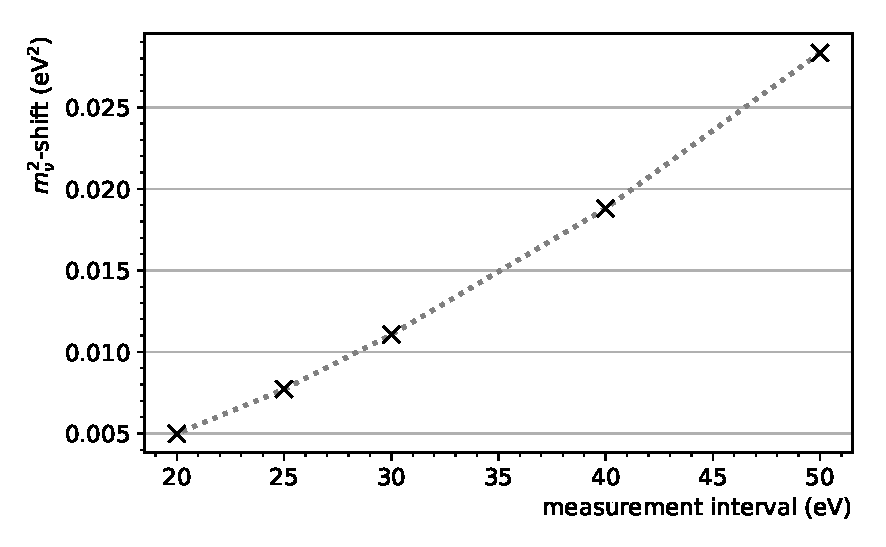
\includegraphics[width=\textwidth]{\currentFigureFolder/nuMassShiftForEDepCrossSec.pdf}
	\xcaption{Shift of an inferred squared neutrino mass induced by a neglected energy-dependence of the inelastic scattering cross section}{Shift of an inferred squared neutrino mass induced by a neglected energy-dependence of the inelastic scattering cross section.}{The neutrino mass was inferred from data that was simulated using an energy-dependent inelastic scattering cross section as per equation~\eqref{eq:eDepScatCrossSecSourcesCrossSecLiu} (with an energy interpretation according to equation~\eqref{eq:eDepScatCrossSecSourcesCrossSecTDREngeryInterpretation} for compatibility with the KATRIN Design Report) and using a nominal four-parameter fit model that assumes a constant cross section of $\sigma_\mathrm{TDR}=\SI{3.456e-22}{m^2}$. The procedure was repeated for five different measurement intervals (respectively \gls{mtd}s) $[E_0-\alpha, E_0+\SI{5}{eV}]$ based on the KATRIN Design Report where $\alpha$ is denoted on the abscissa and $E_0=\SI{18575}{eV}$ is the endpoint of the $\upbeta$ spectrum. The \gls{mtd}s are listed in appendix~\ref{sec:appendixEDepScatCrossSecMTDs}. The markers show the results for the obtained shift of the squared neutrino mass and the dotted line is an interpolation in-between. The study was done once with a free fit parameter for the endpoint and once having it fixed to the simulation truth in order to show the influence on the sign of the shift of the squared neutrino mass (for details refer to the main text).}
	\label{fig:eDepScatCrossSecNuMassInfShifts}
\end{figure}
In the scope of this thesis, an energy-dependent offset of the cross section was investigated (in contrast to a constant one in~\cite{Groh2015}). A KATRIN neutrino mass measurement for a neutrino mass of \SI{0}{eV} was simulated using an energy-dependent cross section\footnote{In all studies presented in this chapter, the simulated electron detector counts were substituted by their expectation values as opposed to fluctuated according to Poissonian statistics. In other words, no ensemble testing was done. For more details on such an Asimov data set and why it can reasonably be assumed to be representative for an ensemble, see section~\ref{sec:katrinElossStatisticsAsimov}.}. A model that uses a constant cross section was fitted to the simulated spectrum. This procedure was repeated for five different \gls{mtd}s of different measurement intervals. Figure~\ref{fig:eDepScatCrossSecNuMassInfShifts} shows the results. For the KATRIN design measurement interval of~\SI{30}{eV}, the difference from \SI{0}{eV}, respectively the shift of the squared neutrino mass, is
\begin{equation}
	\label{eq:eDepScatCrossSecNuMassInfShiftByThisThesis}
	\Delta\nuMass^2 = \SI{1.09e-2}{eV^2}
	\fullstop
\end{equation}
First, it should be noted that this value is greater by a factor of $\sim5$ than the one stated above in equation~\eqref{eq:eDepScatCrossSecNuMassInfShiftEstimate}, that was estimated using the results from~\cite{Groh2015}. This issue is addressed in the subsequent section~\ref{sec:eDepScatCrossSecNuMassInfRelateGrohAndFormerWork}. Further aspects are discussed in the following paragraph:

\paragraph{Sign of the Shift of the Squared Neutrino Mass}
Using an energy-dependent cross section in the simulation and neglecting it in neutrino mass inference yields a higher $\upbeta$ electron count in the endpoint region than expected (see figure~\ref{fig:eDepScatCrossSecNuMassInfIntegralRate}) because the cross section decreases with higher energies and electrons of higher energies are less probable to scatter. On one hand, a higher $\upbeta$ electron count for energies in the endpoint region of the $\upbeta$ spectrum can be caused by a lower squared neutrino mass. On the other hand, a higher $\upbeta$ electron count can also be caused by a higher endpoint of the $\upbeta$ spectrum. These two effects counterbalance each other, which makes it difficult to make an intuitive, qualitative statement about the sign of the shift of the squared neutrino mass. As shown in equation~\eqref{eq:eDepScatCrossSecNuMassInfShiftByThisThesis}, the shift of the squared neutrino mass is positive. However, if the above reasoning is correct, then one should obtain a flip in the sign of the shift if the endpoint is not taken as a free fit parameter, but fixed to the simulation truth. Figure~\ref{fig:eDepScatCrossSecNuMassInfShifts} shows that this is indeed the case.

\paragraph{Significance for the KATRIN Experiment}
The shift of the squared neutrino mass in equation~\eqref{eq:eDepScatCrossSecNuMassInfShiftByThisThesis} takes a sizable fraction of the systematic budget of \SI{1.7e-2}{eV^2} (see eq.~\ref{eq:statMethodsSensitivtyFromEnsembleTDRSysBudget}) of the KATRIN experiment, but is still smaller. Hence, whether the effect of the energy-dependence of the scattering cross section can be neglected depends on the contribution of other systematic effects and can not yet fully be assessed (see for example~\cite{SeitzM2019} for a comprehensive list of systematic effects with regard to the KATRIN experiment).

It should be mentioned that KATRIN's design allows to measure the product of the gas column density and the inelastic scattering cross section $\rho d \cdot \sigma(E)$ for a fixed electron energy~$E$ using the electron gun. In order to respect the energy dependence of the cross section, it is necessary to incorporate a corresponding model, such as the formula for the energy-dependent cross section (eq.~\ref{eq:eDepScatCrossSecSourcesCrossSecLiu}). This might enable the measurement of the two constants $C_1$ and $C_2$ in said formula. Therefore, electron spectra have to be recorded for multiple energies $E$. Such measurements were already conducted at the KATRIN experiment. However, results that respect the energy-dependence of the scattering cross section in the way described here are not yet available at the time of writing this thesis. But a corresponding analysis should be possible.

\subsection{Relation of the Shifts for an Energy-Dependent and -Independent Cross-Section Offset}
\label{sec:eDepScatCrossSecNuMassInfRelateGrohAndFormerWork}
In the scope of this thesis, the shift of an inferred neutrino mass that is introduced by neglecting the energy-dependence of the cross section was investigated. Former works investigated the shift when neglecting a constant offset of the cross section. The shift obtained in this thesis in equation~\eqref{eq:eDepScatCrossSecNuMassInfShiftByThisThesis} is $\sim5$ times larger than the one obtained by the former study in~\cite{Groh2015} under equation~\eqref{eq:eDepScatCrossSecNuMassInfShiftEstimate}, although the energy-dependent offset of the cross section is never greater than the constant offset investigated by~\cite{Groh2015}. This might be contra intuitive, but a possible explanation is the following: The fit parameter for the signal amplitude $\sigAmp$ in a nominal KATRIN fit (see section~\ref{sec:statMethodsStandardFit}) can partly compensate for a constant offset of the cross section. However, it cannot compensate for an energy-dependent one equally well. This is demonstrated below:

The study from~\cite{Groh2015} was reproduced with a free fit parameter for the signal amplitude $\sigAmp$. The reproduced study was in accordance with the values in~\cite{Groh2015}. Then, $\sigAmp=1$ was fixed. The results are shown in figure~\ref{fig:eDepScatCrossSecNuMassInfShiftsForConstCrossSec}. A relative cross section offset of $
\left|
	\Delta\sigma/\sigma_\mathrm{TDR}
\right| \approx \SI{0.1}{\percent}
$ (see equation~\ref{eq:eDepScatCrossSecNuMassInfRelativeCrossSecOffset}) yields a shift of the squared neutrino mass, that is larger by almost an order of magnitude with a fixed $\sigAmp$ as opposed to leaving $\sigAmp$ as a free parameter. The shift is then greater than the one obtained in the study presented in the previous section~\ref{sec:eDepScatCrossSecNuMassInfThisWork} that uses an energy-dependent cross section in the \SI{30}{eV} measurement interval. This verifies, that the fit parameter for the signal amplitude $\sigAmp$ can partly compensate for a constant offset of the cross section. 

Additionally, the following plausibility argument can be given: Figure~\ref{fig:eDepScatCrossSecNuMassInfIntegralRate} shows the simulated integral rate for different cross section models normalized to the integral rate obtained by using the model with a constant cross section $\sigma_\mathrm{TDR}$ from the KATRIN Design Report. The integral rates that are based on a model with a constant, energy-independent cross section differ from each other by almost a constant factor (variations $<2\times10^{-4}$). This implies, when one of these models is used in a simulation of a KATRIN measurement and another model is used in a corresponding fit for neutrino mass inference, their difference can be compensated by the fit parameter for the signal amplitude $\sigAmp$. However, the model that uses an energy-dependent cross section differs from the one with the constant cross section $\sigma_\mathrm{TDR}$ by a factor that varies over the energy range. Such a difference can not be compensated by the fit parameter for the signal amplitude $\sigAmp$.

\begin{figure}[t]
	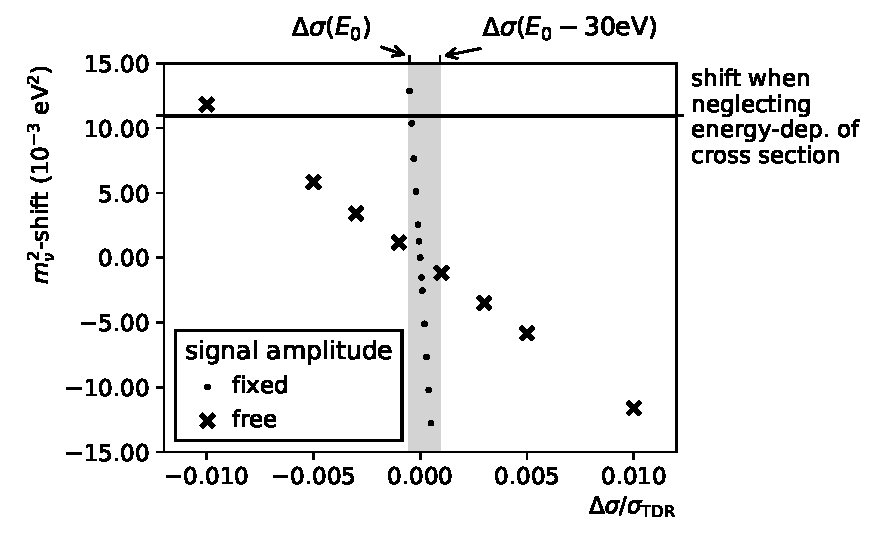
\includegraphics[width=\textwidth]{\currentFigureFolder/nuMassShiftForConstCrossSec.pdf}
	\xcaption{Shift of an inferred squared neutrino mass induced by a neglected constant offset of the inelastic scattering cross section}{Shift of an inferred squared neutrino mass induced by a neglected constant offset of the inelastic scattering cross section.}{The neutrino mass was inferred from data that was simulated using different constant inelastic scattering cross sections. The abscissa shows the offset of the used inelastic scattering cross section relative to $\sigma_\mathrm{TDR}=\SI{3.456e-22}{m^2}$, which was used in the assumed fit model. In an energy-dependent scenario, a cross section corresponds an energy of incident electrons as per equation~\eqref{eq:eDepScatCrossSecSourcesCrossSecLiu}. The cross section range, that corresponds the design KATRIN analysis energy interval of \SI{30}{eV} is depicted as a gray band (energy interpretation as per eq.~\ref{eq:eDepScatCrossSecSourcesCrossSecTDREngeryInterpretation}). The analysis was done twice: once with a free parameter for the signal amplitude, which reproduced the results given in~\cite{Groh2015}~(figure 6.31 on page 221); the second analysis had this parameter fixed. The shift  obtained for $\Delta\sigma/\sigma_\mathrm{TDR}\approx\SI{-0.1}{\percent}$ and a fixed signal amplitude is greater than the shift obtained when neglecting the energy-dependence of the cross section within the \SI{30}{eV} measurement interval (depicted by the horizontal line).}
	\label{fig:eDepScatCrossSecNuMassInfShiftsForConstCrossSec}
\end{figure}


\begin{figure}[t]
	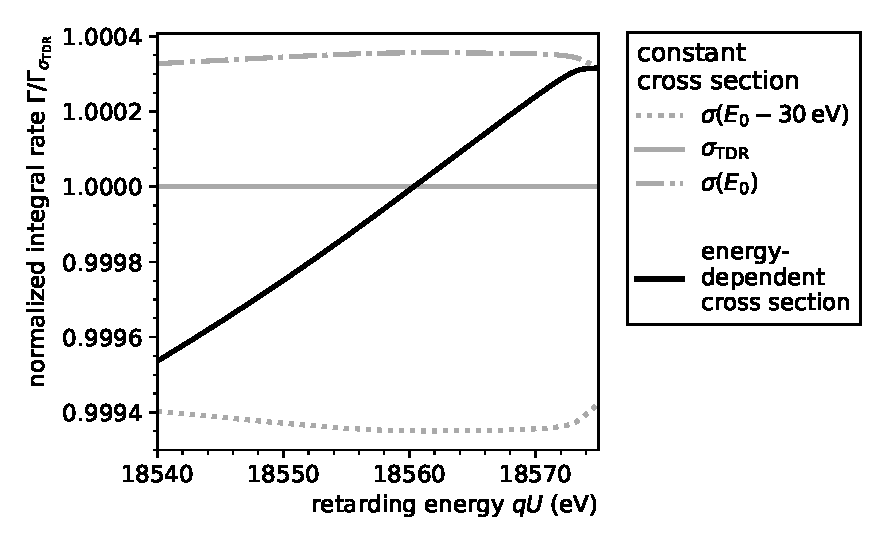
\includegraphics[width=\textwidth]{\currentFigureFolder/normedIntegralRate.pdf}
	\xcaption{Simulated integral $\upbeta$-electron rate using different models of the cross section for inelastic electron-scattering}{Simulated integral $\boldsymbol{\upbeta}$-electron rate using different models of the cross section for inelastic electron-scattering.}{The abscissa shows the energy range of the design KATRIN analysis interval of \SI{30}{eV}. The lines show the integral rate of $\upbeta$~electrons for different models for the inelastic scattering cross section normalized to the model that uses the constant cross section $\sigma_\mathrm{TDR}=\SI{3.456e-22}{m^2}$. The gray lines use a model with a constant cross section. The cross section values can be identified with electron energies as per equation~\eqref{eq:eDepScatCrossSecSourcesCrossSecLiu} and the energy interpretation of equation~\eqref{eq:eDepScatCrossSecSourcesCrossSecTDREngeryInterpretation} with $\sigma(E_0-\SI{30}{eV}=\SI{18545}{eV})=\SI{3.459e-22}{m^2}$ and $\sigma(E_0=\SI{18575}{eV})=\SI{3.454e-22}{m^2}$. The black line shows the simulated integral rate for an energy-dependent cross section. This graph emphasizes that the integral rates for models using a constant cross section differ by an almost constant factor, whereas the rate using an energy-dependent cross section differs from the others by a varying factor.}
	\label{fig:eDepScatCrossSecNuMassInfIntegralRate}
\end{figure}
\FloatBarrier

\section{An Energy-Dependent Scattering Model beyond Using the Poisson Distribution}
\label{sec:eDepScatCrossSecModelExtended}
In the previous section~\ref{sec:eDepScatCrossSecModelPoisson} the scattering probabilities are modeled using a Poisson distribution. This introduces an error for the following reason: A scattering electron loses energy. The scattering cross section increases with decreasing energy (see figure~\ref{fig:eDepScatCrossSecSourcesValues}) and the electron becomes more likely to scatter again. In other words, the probabilities of individual scattering processes are not independent when respecting the dependence on the electron energy. This violates one of the preconditions to model the scattering probabilities via a Poisson distribution. 

This section aims to quantify the error that is introduced by the approximate modeling via a Poisson distribution. Another model is suggested\footnote{The idea was inspired by a model in~\cite{Groh2015} that incorporates changes of the electron pitch angle due to scattering.} in section~\ref{sec:eDepScatCrossSecExtendedModelFormalism} that partly accounts for the energy loss of electrons in the formalism of the scattering probabilities. The suggested model was evaluated numerically as it includes one limit and two integrals that could not yet be solved analytically. The numerical accuracy had to be good enough to decide whether it differs significantly from the Poisson model or not. At the same time, a balance between the numerical accuracy and the evaluation run time had to be found. This matter is described in detail in section~\ref{sec:eDepScatCrossSecExtendedModelNumEval}. The results of the numerical evaluation are discussed in section~\ref{sec:eDepScatCrossSecExtendedModelDiscussion}.

\subsection{Formalism of the Extended Model for Electron-Scattering}
\label{sec:eDepScatCrossSecExtendedModelFormalism}
In the following, a model for the probability of electron-scattering in the \gls{wgts} that depends on the electron energy is derived. The difficulty lies in the fact, that an electron that scatters loses energy and hence its probability to scatter a second time is different from the first time. The presented model assumes the same fixed energy loss $\epsilon$ for each scattering in contrast to a realistic distribution as given by the energy loss function (see figure~\ref{fig:intSpecModelAseevEloss}). This was sufficient to show a difference in the Poisson model and the model suggested below. However, a more accurate description would incorporate the full energy loss function. This may be the subject of a future study. 

The aim of this section is the derivation of an expression $\bar{P}^{\star}_l(\Esource)$ that denotes the probability of $l$-fold scattering for an electron with a starting energy $\Esource$ averaged over all starting positions and pitch angles assuming a fixed energy loss $\epsilon$ per scattering.

The expected amount of scatterings for an electron when traveling through the whole \gls{wgts} volume of length $d$ filled with a gas of constant density $\rho$ is (see equation~\ref{eq:intSpecModelExpectedScatteringCount})
\begin{equation}
\label{eq:eDepScatCrossSecExtendedModelFormalismExpectedScatCount}
\mu(E,\thetaSource) =
\frac{\sigma(E)\rho d}{\cos\thetaSource},
\end{equation}
where $E$ denotes the electron's kinetic energy; $\thetaSource$ the starting pitch angle; and $\sigma(E)$ the energy dependent scattering cross section. It should be noted that the energy $E$ is denoted without and index S here, because, in the following, this formula is reused for different electron energies, not only for the starting energy of an electron.

In the following, the volume of the \gls{wgts} is thought of being divided into $N$ slices of equal width $w=L/N$ (and later the limit $N\rightarrow\infty$ is applied). $N$ is chosen sufficiently large that the probability for an electron to scatter twice within one slice is essentially zero. Then, for large $N$, the probability to scatter within one slice is $\mu(E,\thetaSource)/N$. The probability not to scatter within $n \leq N$ slices is
\begin{equation}
p_0(E,\thetaSource,n) =
\left(
1-\frac{\mu(E,\thetaSource)}{N}
\right)^n
\fullstop
\end{equation}
Let ``Poisson($\mu$,$l$)'' denote the Poisson distribution with expectation value $\mu$ and evaluated at $l$. Using the well known limit for the Euler constant, one obtains for $n=N$ and $N\rightarrow\infty$ that $p_0$ is a Poisson distribution with the expectation value $\mu$ from equation~\eqref{eq:eDepScatCrossSecExtendedModelFormalismExpectedScatCount} and evaluated at $l=0$ 
\begin{align}
\label{eq:eDepScatCrossSecExtendedModelFormalismRecoveryOfPoisson}
\lim_{N\rightarrow\infty} 
p_0(E,\thetaSource,N) =
\lim_{N\rightarrow\infty} 
\left(
1-\frac{\mu(E,\thetaSource)}{N}
\right)^N =
\mathrm{e}^{-\mu(E,\thetaSource)} = 
\mathrm{Poisson}(\mu(E,\thetaSource), 0)
\fullstop
\end{align}
In other words, for no scattering, the Poisson model for the scattering probabilities as described in section~\ref{sec:eDepScatCrossSecModelPoisson} is recovered.

Assuming a constant energy loss $\epsilon$ per scattering, the probability to scatter $l>0$ times within $n<N$ slices can be expressed recursively
\begin{equation}
\label{eq:eDepScatCrossSecExtendedModelFormalismCore}
p_l(E,\thetaSource,n) =
\underbrace{
	\sum_{k=l}^{n}
}_{(4)}
\underbrace{
	p_{l-1}(E,\thetaSource,k-1)
	\vphantom{\sum_{k=l}^{n}}
}_{(1)}
\underbrace{
	\left(
	1-p_0(E-(l-1)\epsilon,\thetaSource,1)
	\right)
	\vphantom{\sum_{k=l}^{n}}
}_{(2)}
\underbrace{
	p_0(E-l\epsilon,\thetaSource,n-k)
	\vphantom{\sum_{k=l}^{n}}
}_{(3)}
\fullstop
\end{equation}
The idea behind this expression is the following: One imagines an electron with an energy $E$ that travels through $n$ \gls{wgts} slices, scatters $l$ times in total and the last time in the $k$th slice. Hence, it must have scattered $l-1$ times in the $k-1$ slices before the $k$th slice and must not scatter in the $n-k$ slices to follow. In that regard, the above expressions have the following meaning:
\begin{enumerate}[(1)]
	\item Probability to scatter $l-1$ times within $k-1$ slices with a kinetic energy of $E$.
	\item Probability to scatter once within the $k$th slice with a kinetic energy of $E-(l-1)\epsilon$.
	\item Probability not to scatter within the remaining $n-k$ slices with a kinetic energy of $E-l\epsilon$.
	\item Sum over all slices $k$ where the electron could scatter the last time. The sum starts at $l$ (as opposed to 1) because the probability to scatter $l-1$ times within less than $k=l-1$ slices (term (1)) is 0 due to the made assumption, that in the limit of a large amount of slices $N$ an electron does not scatter twice within one slice.
\end{enumerate}
The probability to scatter $l$ times can be averaged over all starting positions of electrons respectively starting slices. In this regard, $\nSource$ denotes the amount of slices an electron has to pass through depending on its starting slice (including its starting slice). Then the average is
\begin{equation}
\label{eq:eDepScatCrossSecExtendedModelFormalismZAverage}
\bar{p}_l(E,\thetaSource) = 
\frac{1}{N}
\sum_{\nSource=1}^{N} p_l(E,\thetaSource,\nSource) \approx
\frac{1}{d}
\int_{0}^{d}
p_l(E,\thetaSource,
\left\lceil N \frac{\zSource}{d}\right\rceil
)
\d \zSource
\fullstop
\end{equation}
Here, the averaging sum is approximated by an integral as this helps cutting down on run time in a numerical evaluation. This is due to the fact, that in a numerical evaluation a large number $N$ ($\sim10^5$) of slices has to be chosen and the sum would have many terms. However, a numerical integration can achieve an accurate result with a smaller set of supporting points (see subsequent section~\ref{sec:eDepScatCrossSecExtendedModelNumEval}). 

Then, the limit $N\rightarrow\infty$ can be applied
\begin{equation}
P^{\star}_l(\Esource,\thetaSource) = 
\lim_{N\rightarrow\infty} \bar{p}_l(\Esource,\thetaSource)
\fullstop
\label{eq:eDepScatCrossSecExtendedModelFormalismPitchAngleDepScatProbs}
\end{equation}
$P^{\star}_l(\Esource,\thetaSource)$ denotes the probability for an electron to scatter $l$ times when traveling through the whole \gls{wgts} with a starting energy $\Esource$ and pitch angle $\thetaSource$ averaged over all starting positions. Finally, this expression can be averaged over all starting pitch angles in order to obtain the energy dependent scattering probabilities
\begin{equation}
\bar{P}^{\star}_l(\Esource) = 
\frac{1}{1-\cos\thetaMax}
\int_0^{\thetaMax}
\sin \thetaSource
P^{\star}_l(\Esource,\thetaSource) 
\d \thetaSource
\fullstop
\label{eq:eDepScatCrossSecExtendedModelFormalismAveragedDepScatProbs}
\end{equation}
$\bar{P}^{\star}_l(\Esource)$ denotes the probability for $l$-fold scattering of an electron with a starting energy $\Esource$ averaged over all starting positions and pitch angles assuming a fixed energy loss $\epsilon$ per scattering. In the following, this model is called the ``extended model''.

\subsection{Numerical Accuracy and Cross-Check of the Extended Model for Electron-Scattering}
\label{sec:eDepScatCrossSecExtendedModelNumEval}
\begin{figure}[t]
	\centering
	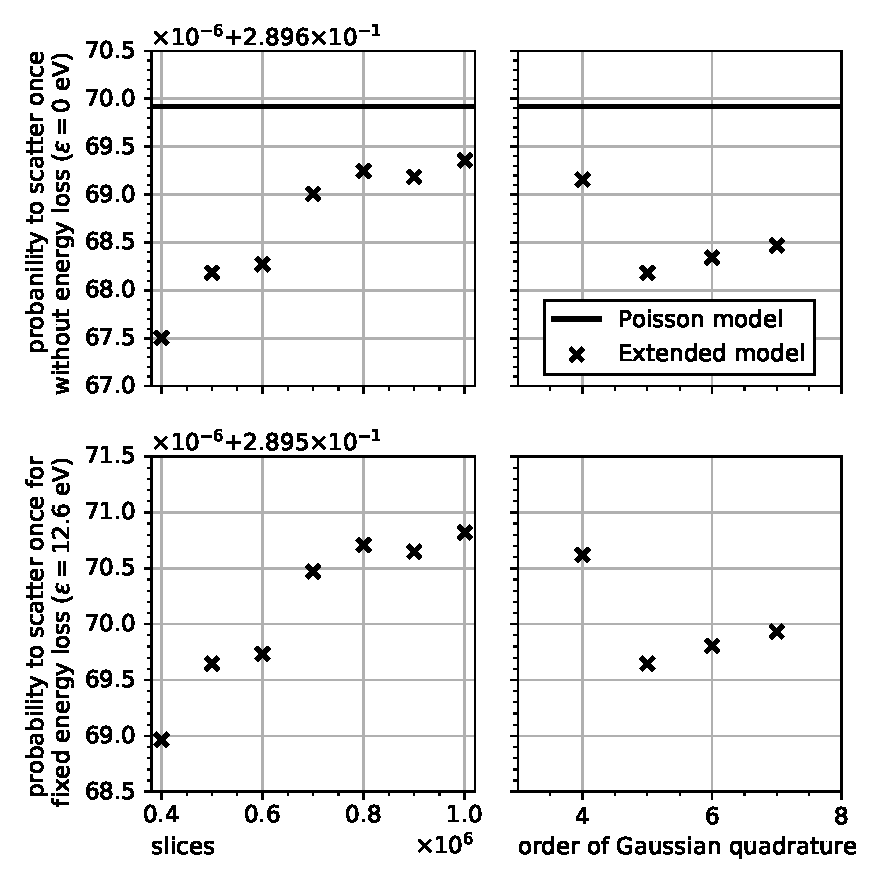
\includegraphics{chapter/energyDependentCrossSec/fig/scatProb1_numericalAccuracy.pdf}
	\xcaption{Accuracy of the numerical evaluation of the extended model of the probability for electron-scattering in the \glsentryshort{wgts}}{Accuracy of the numerical evaluation of the extended model of the probability for electron-scattering in the \glsentryshort{wgts}.}{The extended model is given by equation~\eqref{eq:eDepScatCrossSecExtendedModelFormalismAveragedDepScatProbs} and the Poisson model is given by equation~\eqref{eq:eDepScatCrossSecModelPoisson}. For both models, the energy of the incident electrons was taken such that the Poisson model yields the values already given in table~\ref{tab:eDepScatCrossSecModelScatProbs}. The left column shows the dependence on the number $N$ of slices of the \gls{wgts}. The right column shows the dependence on the order of Gaussian quadrature that was used to evaluate the two integrals in the extended model. The Poisson model is independent of these features and can be evaluated exactly (limited by machine number precision). In the left column, the order of Gaussian quadrature was fixed to 5 and in the right column, the number of slices was fixed to $5\times10^{5}$. The upper row shows the numerical evaluation of the extended model for no energy loss per scattering (markers). Its exact solution is given by the Poisson model (line). The lower row shows the extended model for an energy loss of \SI{12.6}{eV} per scattering. The upper row shows that the numerical evaluation of the extended model is within a distance of less than $3\times10^{-6}$ of its exact solution and the lower row shows convergence on the $10^{-5}$ level. These results make it plausible to assume a numerical accuracy on the $10^{-5}$ level or better for the shown configurations of the numerical evaluation of the extended model.}
	\label{fig:eDepScatCrossSecExtendedModelNumEval}
\end{figure}
For the evaluation of the energy-dependent scattering probabilities according to the extended model in equation~\eqref{eq:eDepScatCrossSecExtendedModelFormalismAveragedDepScatProbs} the fixed energy loss $\epsilon=\SI{12.6}{eV}$ per scattering was chosen as it is the most probable energy loss for electrons traveling through tritium gas (see figure~\ref{fig:intSpecModelAseevEloss}). The mean value would also have been a possible choice. But the energy loss function as depicted in figure~\ref{fig:intSpecModelAseevEloss} is not normalized to $[0, \infty)$, which poses the problem of finding a suitable energy interval, with respect to which the mean value is calculated. In other words, at the current stage, a certain arbitrarity concerning the choice of the energy loss per scattering could not be avoided. As already mentioned, a future study might consider a more comprehensive incorporation of the energy loss function.

The extended model in equation~\eqref{eq:eDepScatCrossSecExtendedModelFormalismAveragedDepScatProbs} was evaluated numerically:
\begin{itemize}
	\item Taking the limit~$N\rightarrow\infty$ in equation~\eqref{eq:eDepScatCrossSecExtendedModelFormalismPitchAngleDepScatProbs} was replaced by choosing a large $N$.
	\item The averaging integral over the starting positions in equation~\eqref{eq:eDepScatCrossSecExtendedModelFormalismZAverage} and starting pitch angles in equation~\eqref{eq:eDepScatCrossSecExtendedModelFormalismAveragedDepScatProbs} were computed using Gaussian quadrature. 
\end{itemize}

The extended model was introduced because the preconditions to model the scattering probabilities via a Poisson distribution (Poisson model) do not hold. Hence, the numerical evaluation of the extended model must be sufficiently accurate to show the difference to the Poisson model. How accurate this is was not known beforehand and was found out by trial and error. Both, $N$ and the order of Gaussian quadrature, should be chosen as low as possible to cut down on calculation run time, but sufficiently high for the required accuracy.

A benchmark had to be found in order to determine the accuracy of the numerical evaluation. The following two ideas were used: First, for an energy loss of $\epsilon=\SI{0}{eV}$ per scattering, the extended model must recover the Poisson model exactly. This can be used to estimate the numerical accuracy in dependence of the number $N$ of slices and order of Gaussian quadrature. The estimated accuracy when using $\epsilon=\SI{0}{eV}$ may then be assumed for evaluations when $\epsilon>\SI{0}{eV}$. Second, a further cross-check is the convergence of the numerical evaluation with increasing $N$ and an increasing order of the Gaussian quadrature. Both ideas find application below.

The averaged probability for one-fold scattering $\bar{P}^{\star}_1$ of the extended model was evaluated for $\epsilon=\SI{0}{eV}$. The result is shown in the top row of figure~\ref{fig:eDepScatCrossSecExtendedModelNumEval} in dependence of $N$ and the order of the Gaussian quadrature. It should recover the Poisson model. For $N=5\times10^5$ and using Gaussian quadrature of order 5, the Poisson model and the extended model differ less than $3\times10^{-6}$. The calculations for $\epsilon=\SI{12.6}{eV}$ are shown in the lower row of figure~\ref{fig:eDepScatCrossSecExtendedModelNumEval}. They also show convergence on the $10^{-5}$ level. Conclusively, the results make it plausible to assume a numerical accuracy on the $10^{-5}$ level or better for $N=10^5$ and using Gaussian quadrature of order 5 for the integrals. Using this configuration, the extended model for one-fold scattering was numerically evaluated for different electron starting energies. The result is depicted in figure~\ref{fig:eDepScatCrossSecExtendedModelResults}. It was found that the extended model and the Poisson model differ by approximately $10^{-4}$. Hence, the numerical accuracy on the $10^{-5}$ level is sufficient to show the difference of these two models.

The corresponding run time to compute $\bar{P}^{\star}_1$ is in $\mathcal{O}(N)$ as it requires a sum over all $N$ slices in equation~\eqref{eq:eDepScatCrossSecExtendedModelFormalismCore}. The extended model is defined recursively and therefore the run time for $l$-fold scattering is in $\mathcal{O}(N^l)$. Hence, computing the probability for two-fold scattering would take $5\times10^5$ times as long as for one-fold scattering for the same $10^{-5}$ accuracy. This was not yet found to be feasible.

The results of the numerical evaluation for one-fold scattering are discussed in the subsequent section~\ref{sec:eDepScatCrossSecExtendedModelDiscussion}.
\FloatBarrier

\subsection{Discussion of the Extended Model for Electron-Scattering}
\label{sec:eDepScatCrossSecExtendedModelDiscussion}
\begin{figure}[t]
	\centering
	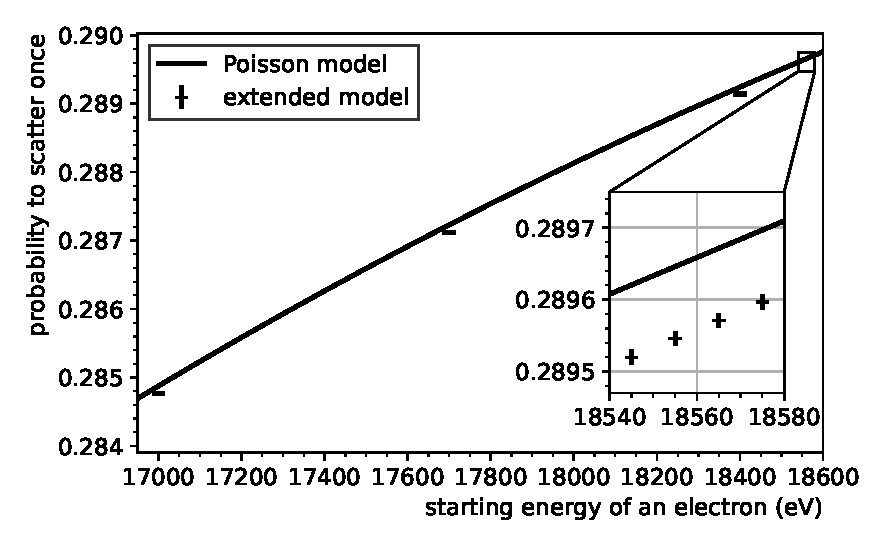
\includegraphics{chapter/energyDependentCrossSec/fig/scatProbs1PoissonAndExtended.pdf}
	\xcaption{Comparison of the Poisson and the extended model for one-fold scattering of electrons in the \glsentryshort{wgts}}{Comparison of the Poisson and the extended model for one-fold scattering of electrons in the \glsentryshort{wgts}.}{The line shows the Poisson model and the markers the extended model (see main text for a description of the models). Due to long program run times, the latter was only evaluated at a selection of energies. Furthermore, the numerical evaluation of the extended model is subject to an error of $\sim10^{-5}$ (see section~\ref{sec:eDepScatCrossSecExtendedModelNumEval}), that is depicted as uncertainty bars. The difference of the two models is $\sim10^{-4}$.}
	\label{fig:eDepScatCrossSecExtendedModelResults}
\end{figure}
For no scattering, the extended model and the Poisson model are equivalent as shown in equation~\eqref{eq:eDepScatCrossSecExtendedModelFormalismRecoveryOfPoisson}.

Figure~\ref{fig:eDepScatCrossSecExtendedModelResults} depicts the Poisson model as per equation~\eqref{eq:eDepScatCrossSecModelPoisson} and the extended model as per equation~\eqref{eq:eDepScatCrossSecExtendedModelFormalismAveragedDepScatProbs} for the probability of one-fold scattering. The difference between the two models is below $10^{-4}$.

For two-fold scattering and higher scattering multiplicities the extended model could not yet be evaluated due to the computational complexity. However an estimation based on theoretical arguments is given below.

\paragraph{Difference of the Extended and the Poisson Model for Electron-Scattering}
The reasoning concerning the sign of the difference between the Poisson and the extended model is similar to the one in section~\ref{sec:eDepScatCrossSecModelPoisson} about the change of the scattering probabilities with decreasing or increasing energy: The Poisson model underestimates the total amount of scattering, because it neglects that an electron that scatters loses energy and becomes more likely to scatter again. As already shown, according to the Poisson model, electrons are expected to scatter between one and two times when traveling through the \gls{wgts} (see equation~\ref{eq:eDepScatCrossSecModelPoissonExpectedScatCount}). The extended model is more correct than the Poisson model and hence should yield an increased expected amount of scattering. Therefore, the probability for one-fold scattering should be smaller than the one given by the Poisson model (this is the case as depicted in figure~\ref{fig:eDepScatCrossSecExtendedModelResults}). For higher scattering multiplicity (which could not be calculated), the sign of the difference between the Poisson and the extended model should be the opposite. In other words, the probability of two-fold scattering as given by the Poisson model should be to low.

Also, the extended model should be a probability distribution and the sum over all scattering multiplicities should yield unity in the same manner as it does for the Poisson model (see appendix~\ref{sec:appendixEDepScatCrossSecPoissonModelProbDensityProof} for a proof that the Poisson model is a probability density). This means that for higher scattering multiplicities, the difference between the extended model and the Poisson model would have to sum up to the difference in the probability for one-fold scattering. Hence, for scattering of higher multiplicity, the absolute difference between the extended model and the Poisson model would not be able to surpass $10^{-4}$.

\paragraph{The Extended Model for Electron-Scattering in Neutrino Mass Inference}
How the error of the Poisson model propagates to neutrino mass inference and whether it would introduce a significant systematic shift of the squared neutrino mass was not probed in the scope of this thesis because the current stage of the extended model is computationally too demanding to be used in a fitting procedure. However, some considerations are given below:

The difference between the extended model and the Poisson model for one-fold scattering is $\sim10^{-4}$, which might be a significant scale because it is similar to the scale on which the probability for one-fold scattering changes when transitioning from an energy-independent to an energy-dependent cross section (see insets of figure~\ref{fig:eDepScatCrossSecModel}). In the previous section~\ref{sec:eDepScatCrossSecNuMassInfThisWork}, it is shown that neglecting such an effect might lead to a systematic shift of the squared neutrino mass on the order of $\SI{e-2}{eV^2}$. Nonetheless, the difference of the extended and the Poisson model might be partly compensated by the different fit parameters such as the signal amplitude or the endpoint of the $\upbeta$ spectrum. Therefore, it was found difficult to make quantifiable assumptions.

In the following, a procedure is outlined, that might make it possible to estimate the induced systematic shift of the squared neutrino mass in a future study: One could simulate data using the Poisson model and additionally introduce an artificial negative shift on the order of $10^{-4}$ on the probability for one-fold scattering and a positive shift that is smaller than $10^{-4}$ for the probability for scattering of higher multiplicities because this should approximately resemble the extended model. The fit model can then use the Poisson model without modification. This procedure might make it possible to quantify whether there is a significant shift of the inferred squared neutrino mass caused by neglecting that electrons become more likely to scatter again if they have already scattered.

\section{Conclusion and Outlook}
\label{sec:eDepScatCrossSecConclusion}
The cross section for inelastic scattering off tritium molecules within the \gls{wgts} depends on the energy of the incident electrons. An approximated model that applies the Poisson distribution (Poisson model) was used to estimate the systematic shift on the squared neutrino mass that would be introduced if the energy-dependence were neglected. The shift would be $\Delta\nuMass^2 = \SI{1.09e-2}{eV^2}$ in a \SI{30}{eV} analysis interval below the endpoint of the $\upbeta$-tritium spectrum. However, the Poisson model can be used in neutrino mass analysis and hence a corresponding systematic shift can be avoided.

It was also shown that including the energy-dependence in neutrino mass inference via the Poisson model increases the run time of the fitting procedure by a factor of up to 140 depending on the \gls{mtd}. A suggestion for an improvement of the performance via interpolation of the scattering probabilities is made in section~\ref{sec:eDepScatCrossSecModelPoissonProperties}.

The usage of the Poisson model underestimates the total amount of scattering because it neglects that an electron that scatters loses energy and becomes more likely to scatter again. This does not influence the probability for no scattering. However, using the approximation of a fixed energy loss $\epsilon=\SI{12.6}{eV}$ per scattering, it could be shown that the probability for one-fold scattering would be shifted by less than $10^{-4}$. The effect on scatterings of higher multiplicities or the effect in neutrino mass inference could not be fully quantified, but an approach that might enable the quantification in the future is outlined in section~\ref{sec:eDepScatCrossSecExtendedModelDiscussion}.

The model building in this chapter was based on well argued considerations. Nonetheless, an independent cross-check is recommended. A future study might perform a Monte Carlo particle tracking simulation in order to verify the suggested models presented in this thesis.
